\documentclass[11pt]{article}
\usepackage[utf8]{inputenc}
\usepackage[T1]{fontenc}
\usepackage{amsmath}
\usepackage{amssymb} % Needed for \eth if used, though not in L7
\usepackage{graphicx}
\usepackage{geometry}
\usepackage{tikz}
\usepackage{pgfplots} % For plots
\usepackage{ulem}     % For underline, using normalem to avoid messing with \emph

\geometry{a4paper, margin=1in}
\usetikzlibrary{positioning, arrows.meta, shapes.geometric} % For TikZ diagrams
\pgfplotsset{compat=1.18} % Use a recent PGFPlots version

% Custom commands (optional)
\newcommand{\avg}[1]{\overline{#1}}
\newcommand{\prob}[1]{P(#1)}
\newcommand{\ProbDens}[1]{\mathcal{P}(#1)} % Using script P for density
\newcommand{\vect}[1]{\vec{#1}}
\newcommand{\dd}[1]{\mathrm{d}#1} % Differential d
\newcommand{\pderiv}[2]{\frac{\partial #1}{\partial #2}}
\newcommand{\deriv}[2]{\frac{\mathrm{d} #1}{\mathrm{d} #2}}
\newcommand{\muState}{\mu\text{-state}} % Microstate
\newcommand{\OmegaE}{\Omega(E)}
\newcommand{\omegaE}{\omega(E)}
\newcommand{\PhiE}{\Phi(E)}
\newcommand{\deltaE}{\delta E}
\newcommand{\ethbar}{\text{\it{đ}}} % \eth symbol for inexact differential
\newcommand{\kb}{k_B} % Boltzmann constant

\title{Physics 415 - Lecture 7: Statistical Thermodynamics}
\date{February 5, 2025}
\author{} % Author not specified

\begin{document}

\maketitle
\thispagestyle{empty}

Connect statistical mechanics with general properties of macroscopic systems. Introduce important (purely statistical) notions of entropy \& temperature.

\section*{Recap}
\begin{itemize}
    \item Isolated system with energy in range $(E, E+\deltaE)$.
    \item $\OmegaE = \#$ of accessible $\mu$-states.
    \item Fundamental Postulate: In equilibrium, Prob($\muState$) $= 1/\OmegaE$.
    \item Equilibrium $\implies$ probability distribution of $\mu$-states is time-independent.
\end{itemize}

\section*{Interaction Between Macroscopic Systems: Thermal Contact}

Consider two macroscopic systems, 1 and 2, which can exchange energy through heat transfer (thermal contact). Assume no work is done for now (e.g., volumes $V_1, V_2$ fixed).

\begin{center}
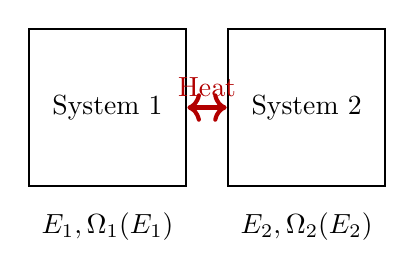
\begin{tikzpicture}
    \node (A) [draw, thick, minimum width=2cm, minimum height=2cm, label=center:System 1] {};
    \node (B) [draw, thick, minimum width=2cm, minimum height=2cm, right=0.5cm of A, label=center:System 2] {};
    % Interface allowing heat exchange
    \draw [line width=1.5pt, red!70!black, <->] (A.east) -- (B.west) node [midway, above] {Heat};
    % Properties
    \node at (A.south) [below=0.2cm] {$E_1, \Omega_1(E_1)$};
    \node at (B.south) [below=0.2cm] {$E_2, \Omega_2(E_2)$};
\end{tikzpicture}
\end{center}

\begin{itemize}
    \item The combined system (1+2) is isolated. Total energy $E = E_1 + E_2 = \text{constant}$.
    \item Assume interaction between 1 \& 2 is weak enough that energy is additive.
    \item Now, $E$ is fixed, but $E_1$ and $E_2$ can vary ($E_2 = E-E_1$) due to energy exchange.
    \item In a statistical ensemble of such combined systems, there will be a distribution of values for $E_1$ (and $E_2$).
\end{itemize}
The number of accessible states of the combined system when system 1 has energy $E_1$ (and system 2 has $E_2=E-E_1$) is $\Omega_1(E_1) \Omega_2(E-E_1)$.
The total number of accessible states of the combined system is:
\[ \Omega(E) = \sum_{E_1} \Omega_1(E_1) \Omega_2(E-E_1) \]
(The sum is over all possible energies $E_1$ of system 1).

The probability that system 1 has energy $E_1$ is:
\[ P_1(E_1) = \frac{\text{\# states where system 1 has } E_1}{\text{Total \# states}} = \frac{\Omega_1(E_1) \Omega_2(E-E_1)}{\Omega(E)} \]

Now investigate how $P_1(E_1)$ behaves for a macroscopic system.
Recall $\Omega(E) \sim E^{aN}$, where $N=$ \# of particles and $a \sim O(1)$ (e.g., $a=3N/2$ for classical ideal gas). $\Omega$ grows extremely rapidly with $E$ and $N$.
Schematically: $\Omega_1(E_1) \sim E_1^{a_1 N_1}$ and $\Omega_2(E_2) = \Omega_2(E-E_1) \sim (E-E_1)^{a_2 N_2}$.
The product $\Omega_1(E_1) \Omega_2(E-E_1)$ will be very sharply peaked around some value $E_1 = \tilde{E}_1$.

\begin{center}
\begin{tikzpicture}
\begin{axis}[
    axis lines=left, xlabel=$E_1$, ylabel=$P_1(E_1)$,
    xtick=\empty, ytick=\empty,
    ymax = 1.2, % Adjust ymax to fit peak
    samples=101, smooth
]
\addplot [domain=0:5, thick, blue] {exp(-10*(x-2.5)^2)}; % Gaussian representing sharp peak
\draw [dashed] (axis cs:2.5, 0) -- (axis cs:2.5, 1) node[pos=1.1, above] {$\tilde{E}_1$};
\node at (axis cs:2.5, 0) [below] {Most Probable Energy};
\draw [<->] (axis cs:2.2, 0.1) -- (axis cs:2.8, 0.1) node[midway, below] {Width $\Delta^* E_1 \ll \tilde{E}_1$};
\end{axis}
\end{tikzpicture}
\end{center}

The probability $P_1(E_1)$ is narrowly peaked near the most probable value $E_1 = \tilde{E}_1$. The width $\Delta^* E_1$ of the peak is very small compared to $\tilde{E}_1$ for macroscopic systems.

Let's find the most probable value $\tilde{E}_1$ by finding the maximum of $P_1(E_1)$. It's easier to maximize $\ln P_1(E_1)$:
\[ \ln P_1(E_1) = \ln \Omega_1(E_1) + \ln \Omega_2(E-E_1) - \ln \Omega(E) \]
Set the derivative with respect to $E_1$ to zero:
\[ \pderiv{}{E_1} (\ln P_1(E_1)) = \pderiv{(\ln \Omega_1)}{E_1} + \pderiv{(\ln \Omega_2)}{E_1} - 0 = 0 \]
Using the chain rule for the second term: $\pderiv{}{E_1} = \pderiv{E_2}{E_1} \pderiv{}{E_2} = (-1) \pderiv{}{E_2}$.
\[ \pderiv{(\ln \Omega_1)}{E_1} - \pderiv{(\ln \Omega_2)}{E_2} = 0 \]
\[ \implies \left. \pderiv{(\ln \Omega_1)}{E_1} \right|_{E_1=\tilde{E}_1} = \left. \pderiv{(\ln \Omega_2)}{E_2} \right|_{E_2=E-\tilde{E}_1} \qquad (*) \]
This condition determines the most probable energy distribution $(\tilde{E}_1, \tilde{E}_2)$.

\section*{Entropy and Temperature}

We define the (statistical) "entropy" $S$ as:
\[ S \equiv \ln \Omega \]
(Note: We will discuss units involving Boltzmann's constant $k_B$ later. For now, $S$ is dimensionless).

The condition $(*)$ for the most probable energy distribution becomes:
\[ \left. \pderiv{S_1}{E_1} \right|_{\tilde{E}_1} = \left. \pderiv{S_2}{E_2} \right|_{\tilde{E}_2} \]
This is the condition that determines the energy sharing $(\tilde{E}_1, \tilde{E}_2)$ when the systems are in thermal equilibrium.

Also note that maximizing $P_1(E_1)$ is equivalent to maximizing $\ln P_1(E_1) = S_1 + S_2 - \ln \Omega(E)$. Since $\Omega(E)$ is constant, this is equivalent to maximizing the total entropy $S = S_1 + S_2$.
The condition of maximum probability = condition of maximum total entropy.

The quantity $\partial S / \partial E$ is clearly important. We define the "absolute temperature" $T$ such that:
\[ \frac{1}{T} \equiv \pderiv{S}{E} \]
(Note: With $S = \ln \Omega$, $T$ has units of energy).
The condition for thermal equilibrium between systems 1 and 2 is then simply:
\[ \frac{1}{T_1} = \frac{1}{T_2} \implies T_1 = T_2 \]

\textbf{Question:} How do we identify $T = 1/(\partial S/\partial E)$ with the familiar notion of temperature?
We'll show that this quantity $T$ behaves qualitatively as you'd expect for temperature. Consider how systems 1 and 2 approach equilibrium.

\subsection*{Approach to Equilibrium}

Consider the initial situation where 1 and 2 are thermally isolated with initial mean energies $\avg{E}_1^{(0)}$ and $\avg{E}_2^{(0)}$, and corresponding initial temperatures $T_1^{(0)}$ and $T_2^{(0)}$. Assume $T_1^{(0)} \neq T_2^{(0)}$.
Now, suppose the insulating barrier is removed, so energy can be exchanged (heat transfer).
We expect the mean energies to evolve in time toward the most probable state $\tilde{E}_1, \tilde{E}_2$. Since $P_1(E_1)$ is sharply peaked, we can identify the final average energies with the most probable energies: $\avg{E}_1 \to \tilde{E}_1$ and $\avg{E}_2 \to \tilde{E}_2$. (Conservation holds: $E_1^{(0)}+E_2^{(0)} = \tilde{E}_1+\tilde{E}_2 = E$).

Consider the rate of change of total entropy $S = S_1(E_1) + S_2(E_2)$ as the systems evolve (assume evolution is slow enough to define $S_1, S_2$ at each step, i.e., quasi-static approach):
\[ \deriv{S}{t} = \deriv{S_1}{t} + \deriv{S_2}{t} = \pderiv{S_1}{E_1} \deriv{E_1}{t} + \pderiv{S_2}{E_2} \deriv{E_2}{t} \]
Since $E_1+E_2=E=$ const, $\deriv{E_2}{t} = -\deriv{E_1}{t}$.
\[ \deriv{S}{t} = \left( \pderiv{S_1}{E_1} - \pderiv{S_2}{E_2} \right) \deriv{E_1}{t} \]
Using the definition $1/T = \partial S / \partial E$:
\[ \deriv{S}{t} = \left( \frac{1}{T_1} - \frac{1}{T_2} \right) \deriv{E_1}{t} \]
Now, suppose initially $T_2^{(0)} > T_1^{(0)}$. We expect heat to flow from the hotter system (2) to the colder system (1). This means system 1 gains energy, so $\deriv{E_1}{t} > 0$.
In this case, since $T_2 > T_1 \implies 1/T_1 > 1/T_2$, the term $(1/T_1 - 1/T_2)$ is positive.
Therefore, $\deriv{S}{t} > 0$.
The total entropy $S$ increases until equilibrium is reached, where $T_1=T_2$ and $dS/dt=0$.

This demonstrates a key aspect of the Second Law of Thermodynamics: For an isolated system (1+2), the entropy tends to increase towards its maximum value, which corresponds to equilibrium. It also shows that energy passes (heat is transferred) from the system at higher $T$ to that at lower $T$, consistent with our intuitive understanding of temperature.

\subsection*{Some Additional Properties of T}

Since $\OmegaE \sim E^{aN}$ (in general for large $N$), we have $S = \ln \Omega \sim aN \ln E$.
Then $\frac{1}{T} = \pderiv{S}{E} \sim \frac{aN}{E}$.
\[ \implies T \sim \frac{E}{aN} \]
We also expect $E$ to be positive, and $\Omega$ increases with $E$, so $\partial S/\partial E > 0$, which means $T>0$ (generally).
The temperature $T$ measures (roughly) the mean energy per degree of freedom (or per particle) for the system.
When two systems are in thermal contact, the equilibrium condition $T_1=T_2$ is therefore (roughly) the statement that the total energy $E=E_1+E_2$ is shared between the systems such that the mean energy per DOF is the same for both systems.

\section*{Note on Units}

We have defined $T$ with units of energy (since $1/T = \partial S / \partial E$ and $S=\ln\Omega$ is dimensionless).
Often, temperature is measured in degrees Kelvin (K). The conversion factor is Boltzmann's constant:
\[ k_B \approx 1.38 \times 10^{-23} \, \text{J/K} \quad (\text{or } 1.38 \times 10^{-16} \, \text{erg/K}) \]
\[ T_{\text{energy}} = k_B \times T_{\text{Kelvin}} \]
If temperature $T$ is measured in degrees (Kelvin), a factor of $k_B$ is also conventionally included in the definition of entropy to make the argument of functions like $\exp(-E/(\kb T))$ dimensionless:
\[ S_{\text{conventional}} = k_B \ln \Omega \]
This gives $S$ units of Energy/Temperature (e.g., J/K).
$\pderiv{S_{\text{conv}}}{E} = k_B \pderiv{(\ln \Omega)}{E} = k_B \left( \frac{1}{T_{\text{energy}}} \right) = \frac{k_B}{k_B T_{\text{Kelvin}}} = \frac{1}{T_{\text{Kelvin}}}$.
The definition $1/T = \partial S/\partial E$ holds regardless of the units chosen for $T$, provided $S$ is defined consistently.

We will often (unless specified otherwise) measure $T$ in energy units and keep $S = \ln \Omega$ dimensionless. To convert results to conventional units, make the substitutions $T \to \kb T$ and $S \to S/\kb$.

\end{document}